% 1) Title
% 2) Date
% 3) Location
% 4) Present
% 5) Picture
% 6) Start Time
% 7) Stop Time
\insertmeeting 
	{Some Light Learning} 
	{08/31/21}
	{Hagerty High School}
	{Anouska, James, Jensen, Samantha}
	{Images/RobotPics/robot.jpg}
	{2:30}
  {4:30}
	
\section*{Hardware}
\noindent\hfil\rule{\textwidth}{.4pt}\hfil
\subsection*{Goals}
\begin{itemize}
    \item Help newer members learn onshape’s custom features and assemblies
  

\end{itemize} 

\noindent\hfil\rule{\textwidth}{.4pt}\hfil

\subsection*{Accomplishments}
At the meeting today, we wanted to work on expanding some of our newer member’s knowledge of CAD. Because we want our members to have some experience in every skill that we use, we thought now, before the game is revealed, would be the best time to start learning CAD. Because the two members that we were working with today had already learned how to make sketches, we wanted to focus more on using custom features and creating an assembly. We decided to have them follow along with one of our older Hardware committee members who would show them how to make a wood box with box joints and t-slot joints. We started out by downloading the box joint and t-slot joint custom features. From there, we had them sketch and extrude the first 3 sides of the box without any box joints or t-slot joints (image 1). After that, we showed the learning members the mirror tool, using it to mirror two of the sides of the box so that we had a 5 sided box (image 2). We finished up all of the box’s parts by adding box joints and t-slot joints into the plates, just like we do on our robot’s parts. 
From there, we created an assembly where the newer members were shown how the fasten mate works by putting the parts of the box together. Although the box still looked the same as in the part studio, mating parts together in assemblies is a very important part of CAD. To add to this knowledge, we showed them how to insert standard content, like 6-32 screws into their CAD (image 3). Although we ran out of time to show the other types of mates, we were able to cover the fasten mate well, which is the most commonly used type of mate. Overall the newer members’ CAD skills have been progressing very quickly, and they seem well equipped for the upcoming season. Next is to continue teaching less experienced CAD members other types of mates
and demonstrating more complicated skeletons. 


\begin{figure}[ht]
\centering
\begin{minipage}[b]{.50\textwidth}
  \centering
  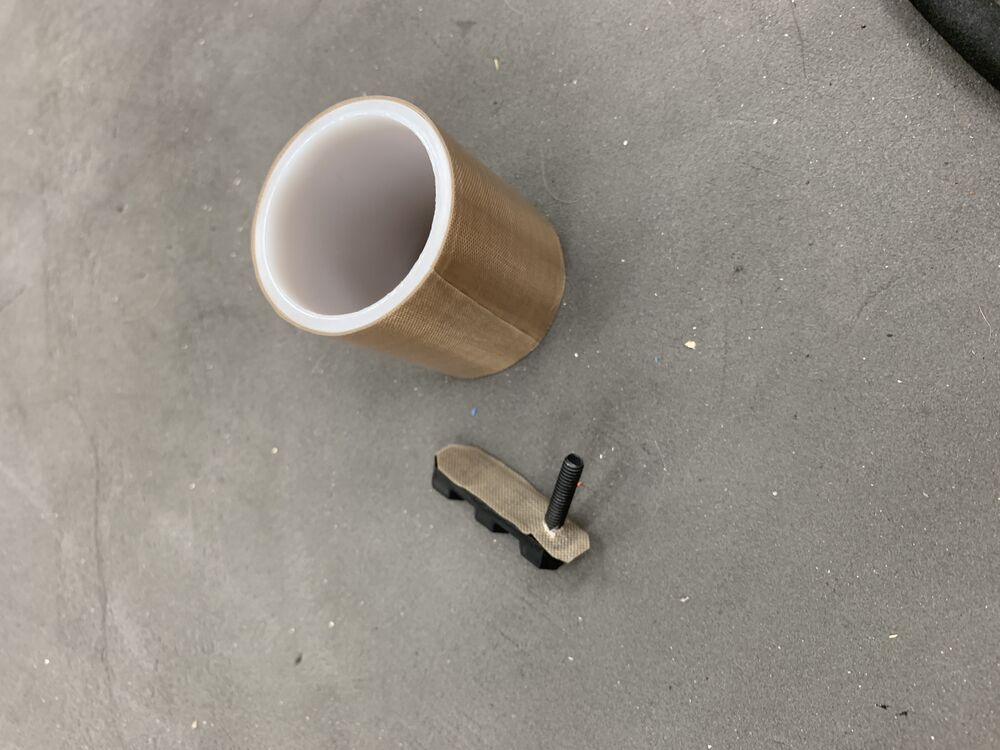
\includegraphics[width=0.8\textwidth]{Meetings/August/08-18-21/8-26-21_Hardware_Image1 - Nathan Forrer.JPG}
  \caption{Our bearing blocks covered in Teflon to reduce friction with the plates.}
  \label{fig:pic1}
\end{minipage}%
\hfill%
\begin{minipage}[b]{.50\textwidth}
  \centering
  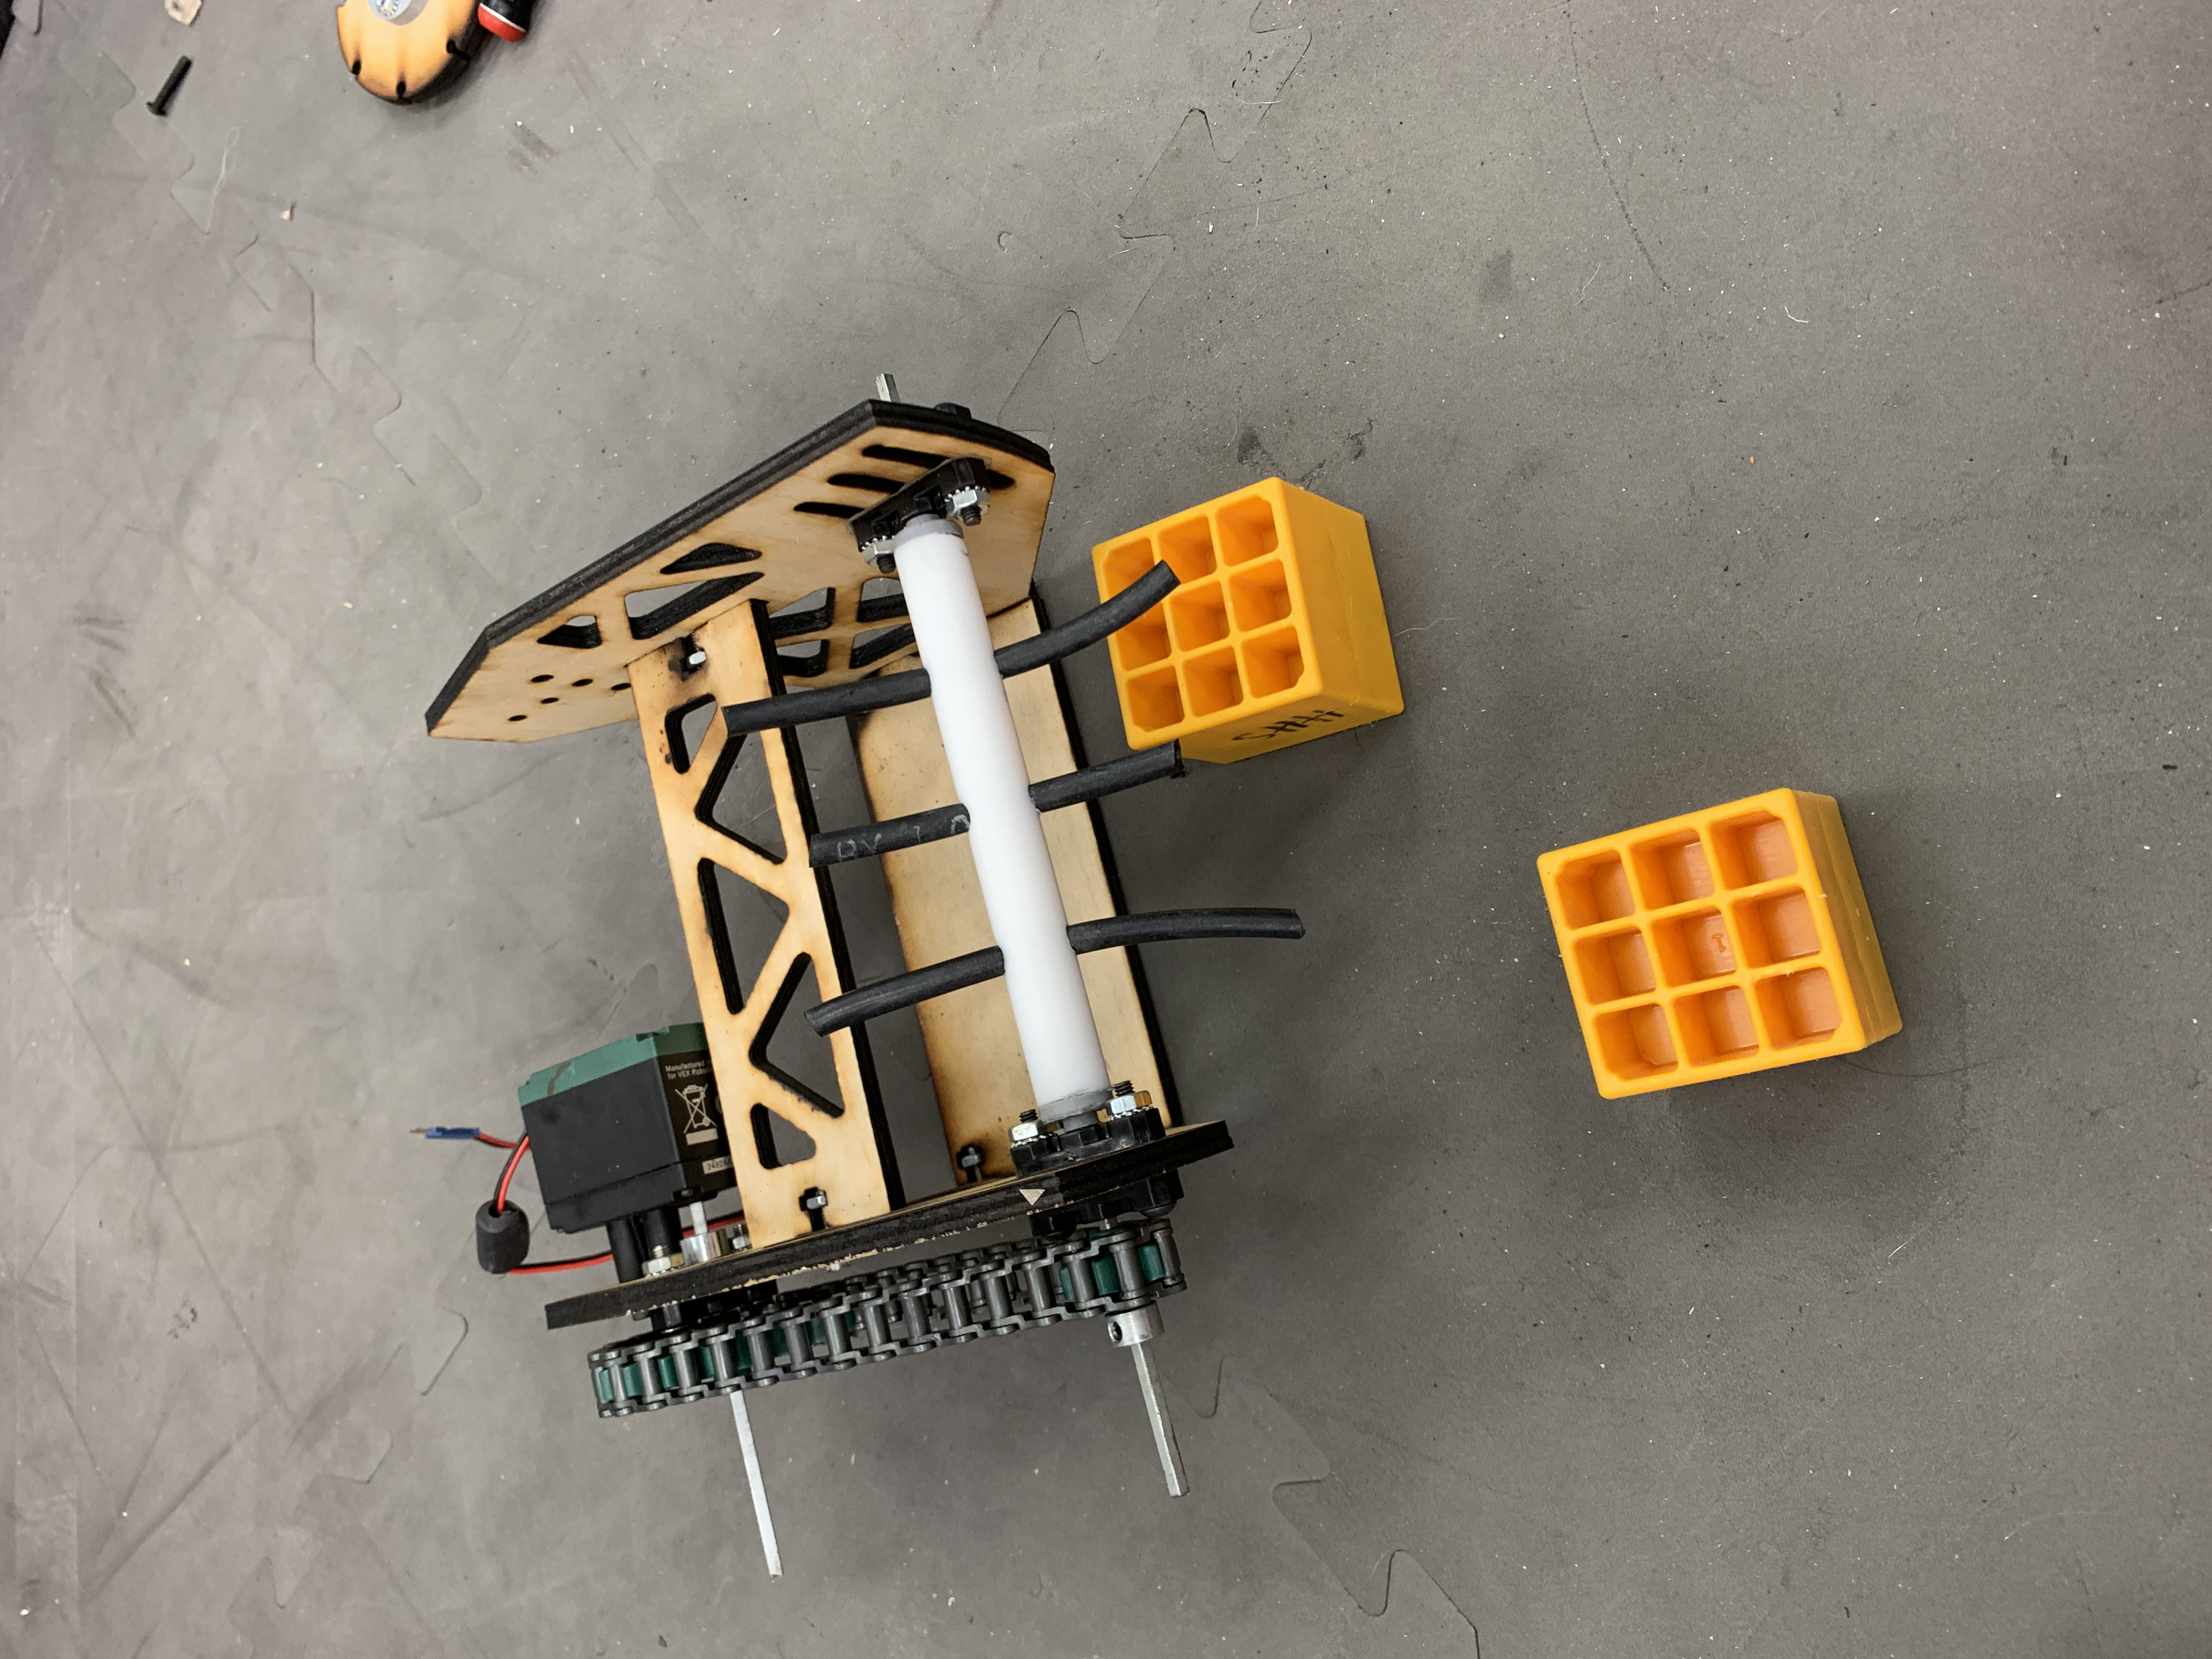
\includegraphics[width=0.8\textwidth]{Meetings/August/08-18-21/8-26-21_Hardware_Image2 - Nathan Forrer.JPG}
  \caption{Our second version of the intake uses a tube sweeper instead of the rubber band spinner.}
  \label{fig:pic2}
\end{minipage}
\end{figure}

\begin{figure}[htp]
\centering
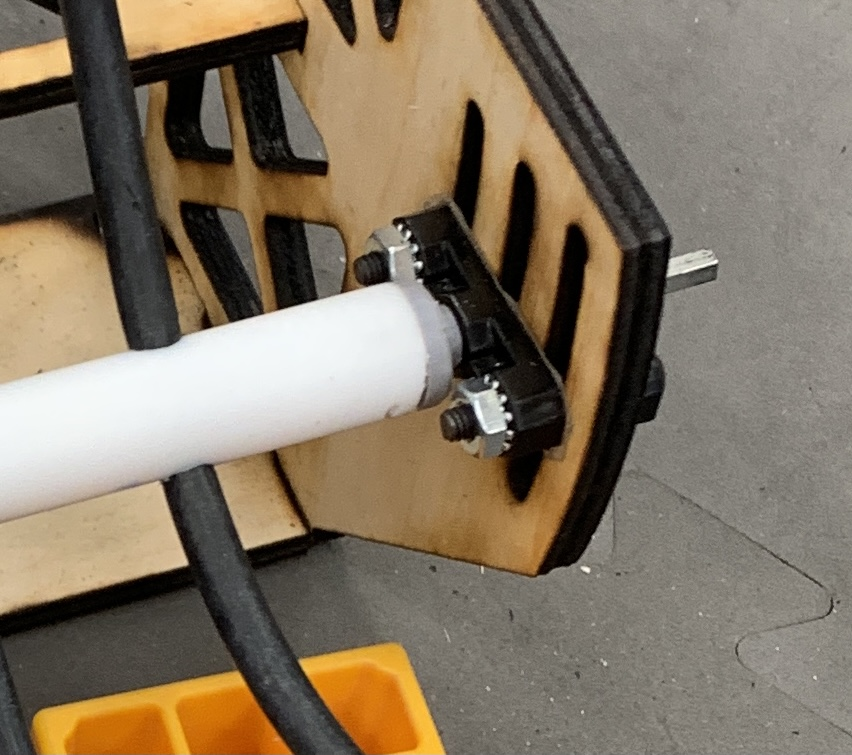
\includegraphics[width=0.8\textwidth]{Meetings/August/08-18-21/8-26-21_Hardware_Image3 - Nathan Forrer.JPG}
\caption{We got better results when tightening the nuts higher than expected.}
\label{fig:pic3}
\end{figure}